\section{Chiusure}
Come gi\`a osservato nell'esempio introduttivo, il modello botton-up su una rete richiede un elevato numero di equazioni differenziali: le equazioni per i nodi dipendono dalle coppie, le coppie dalle triple e cos\`i via.\\
Tale approccio, al crescere del numero di nodi, risulterebbe computazionalmente intrattabile. Per risolvere questo problema dobbiamo trovare alcune semplificazioni che ci permettono di esprimere le coppie in termini dei singoli nodi, le triple in termini delle coppie e dei nodi e cos\`i via.\\
Se riusciamo a fare ci\`o, possiamo rompere la ``cascata" nella quale ogni struttura dipende da tutte le strutture di ordine superiore.\\ \\
Andiamo a presentare un approccio formale basato sul lavoro di Keeling~\cite{keeling1995ecology}  e van Baalen~\cite{van2000pair}.  A tal fine introduciamo i  \textit{coefficienti di correlazione}.\\
Siano $A, B\in \{ S, I,R\}$ e $(i,j)\in E$ allora 
$$C_{A_i B_j} = \frac{\angol{A_i B_j}}{\angol{A_i} \angol{B_j}}.$$
Tali coefficienti quantificano la propensione che due nodi adiacenti abbiamo stato differente o identico.\\
Se $C_{A_iB_j}=1$ allora possiamo, in modo equivalente, assuemere  $A_i$ e $B_j$ indipendenti.\\
Osserviamo che nel modello $SIR$ gli stati non sono per\`o indipendenti. I nodi infetti possono infettare i loro vicini dunque hanno una maggior probabilit\`a di essere uniti ad altri nodi infetti,  di conseguenza  $C_{I_i I_j}\geq 1$.  Diremo che $I_i$ e $I_j$ sono correlati positivamente.\\
Con medesime argomentazioni si arriva a dire che $S_i$ e $I_j$ sono correlati negativamente: $C_{S_i I_j}\leq 1$.\\
 In un certo senso, sapere che $j$ \`e infetto aumenta la nostra aspettativa  che $i$ sia infetto e diminuisce quella che sia sano.\\
 
\subsection{Chiusura al livello delle coppie}
Da quanto osservato nella parte introduttiva sulle chiusure, possiamo scrivere:
$$ \angol{ A_i B_j} = \angol{ A_i} \angol{B_j} C_{A_i B_j} \text{ dove } A,B\in \{S,I,R\} \text{ e } (i,j)\in E.$$ 
Assumendo, in prima approssimazione, l'indipendenza a livello delle coppie abbiamo 
$$ \angol{ A_i B_j} \approx \angol{A_i}\angol{B_j}.$$ 
Per enfatizzare che non abbiamo identit\`a esatte, quando andremo a risolvere un sistema ottenuto usando le chiusure denoteremo  con $\angol{X_i}$ l'approssimazione di $\angol{ S_i}$ e con $\angol{ Y_i}$ quella di $\angol{ I_i}$.\\ \\
Presentiamo il modello botton-up generale su una rete con $N$ nodi senza loop e mostriamo come usando l'indipendenza a livello delle coppie si riesca ad ottenere un sistema di equazioni differenziali chiuse.\\
Sia $G=(g_{ij})$ la matrice di adiacenza del grafo $G$. Assumiamo che il tasso di trasmissione da $i$ a $j$ sia $\tau g_{ij}$ e che il tasso di rimozione per il nodo $i$ sia $\gamma_i$ indipendentemente dallo stato di ogni altro nodo.\\
Dunque le equazione per il sistema diventano
\begin{equation}
\begin{aligned}
	 \angol{ S_i} =& -\tau \sum_{j=1\atop{j\neq i }}^N\angol{ S_i I_j},\\
	 \angol{I_i} =&\spa \tau \sum_{j=1\atop{j\neq i}}^N \angol{ S_i I_j} -\gamma_i \angol{I_i},
\end{aligned}
\end{equation}
dove ricordiamo che $\angol{R_i}=1-\angol{S_i}- \angol{I_i}$.\\
Usando l'indipendenza a livello delle coppie possiamo un sistema chiuso: 
\begin{equation}
\begin{aligned}
	 \angol{ X_i} =& -\tau \sum_{j=1\atop{j\neq i }}^N\angol{ X_i} \angol{Y_j},\\
	 \angol{Y_i} =&\spa \tau \sum_{j=1\atop{j\neq i}}^N \angol{ X_i}\angol{Y_j} -\gamma_i \angol{Y_i}.
\end{aligned}
\label{Coppie3nodi}
\end{equation}
Nella Figura~\ref{fig::coppie3nodi} possiamo confrontare le soluzioni del modello esatto con l'approssimazione ottenuta  dall'indipendenza a livello delle coppie per il grafo~\ref{fig::3nodi}. Per non appesantire i grafici abbiamo tracciato solamente  $\angol{S_i}$ e $\angol{I_i}$ in funzione  del tempo: $\angol{ R_i}$ pu\`o essere ricavata.
\begin{figure}[!h]

\centering
\subfloat[][Nodo 1]
{\resizebox{0.45\textwidth}{!}{% This file was created by matlab2tikz.
%
%The latest updates can be retrieved from
%  http://www.mathworks.com/matlabcentral/fileexchange/22022-matlab2tikz-matlab2tikz
%where you can also make suggestions and rate matlab2tikz.
%
\begin{tikzpicture}

\begin{axis}[%
width=6.028in,
height=4.754in,
at={(1.011in,0.642in)},
scale only axis,
xmin=0,
xmax=5,
ymin=0,
ymax=1,
axis background/.style={fill=white},
axis x line*=bottom,
axis y line*=left,
legend style={legend cell align=left, align=left, draw=white!15!black}
]
\addplot [color=blue, dashed, line width=2.0pt]
  table[row sep=crcr]{%
0	0\\
0.000100475457260383	0\\
0.000200950914520766	0\\
0.00030142637178115	0\\
0.000401901829041533	0\\
0.000904279115343449	0\\
0.00140665640164536	0\\
0.00190903368794728	0\\
0.0024114109742492	0\\
0.00492329740575878	0\\
0.00743518383726836	0\\
0.00994707026877794	0\\
0.0124589567002875	0\\
0.0250183888578354	0\\
0.0375778210153833	0\\
0.0501372531729312	0\\
0.0626966853304791	0\\
0.0991412937643315	0\\
0.135585902198184	0\\
0.172030510632036	0\\
0.208475119065889	0\\
0.257093885813804	0\\
0.305712652561719	0\\
0.354331419309635	0\\
0.40295018605755	0\\
0.46627950019307	0\\
0.52960881432859	0\\
0.592938128464109	0\\
0.656267442599629	0\\
0.733658471248229	0\\
0.811049499896829	0\\
0.888440528545428	0\\
0.965831557194028	0\\
1.05793596976172	0\\
1.15004038232942	0\\
1.24214479489711	0\\
1.3342492074648	0\\
1.44286725998794	0\\
1.55148531251107	0\\
1.66010336503421	0\\
1.76872141755734	0\\
1.88893196521442	0\\
2.00914251287149	0\\
2.12935306052856	0\\
2.24956360818563	0\\
2.37456360818563	0\\
2.49956360818563	0\\
2.62456360818563	0\\
2.74956360818563	0\\
2.87456360818563	0\\
2.99956360818563	0\\
3.12456360818563	0\\
3.24956360818563	0\\
3.37456360818563	0\\
3.49956360818563	0\\
3.62456360818563	0\\
3.74956360818563	0\\
3.87456360818563	0\\
3.99956360818563	0\\
4.12456360818563	0\\
4.24956360818563	0\\
4.37456360818563	0\\
4.49956360818563	0\\
4.62456360818563	0\\
4.74956360818563	0\\
4.81217270613922	0\\
4.87478180409282	0\\
4.93739090204641	0\\
5	0\\
};
\addlegendentry{$\langle\text{ S}_\text{1}\rangle\text{(t)}$}

\addplot [color=blue, dashdotted, line width=2.0pt]
  table[row sep=crcr]{%
0	1\\
0.000100475457260383	0.999899530851975\\
0.000200950914520766	0.999799074321068\\
0.00030142637178115	0.999698630405252\\
0.000401901829041533	0.999598199102498\\
0.000904279115343449	0.999096231713726\\
0.00140665640164536	0.998594579347576\\
0.00190903368794728	0.998093241751005\\
0.0024114109742492	0.997592218671205\\
0.00492329740575878	0.995091812191547\\
0.00743518383726836	0.992599230844247\\
0.00994707026877794	0.99011444329054\\
0.0124589567002875	0.987637418335814\\
0.0250183888578354	0.975367649924921\\
0.0375778210153833	0.963287349850503\\
0.0501372531729312	0.95139277818569\\
0.0626966853304791	0.939680278465966\\
0.0991412937643315	0.906691121197265\\
0.135585902198184	0.875122026261053\\
0.172030510632036	0.84489505392913\\
0.208475119065889	0.815936847771523\\
0.257093885813804	0.779162082786105\\
0.305712652561719	0.744374033314346\\
0.354331419309635	0.711435438681249\\
0.40295018605755	0.680218977306833\\
0.46627950019307	0.641947443142085\\
0.52960881432859	0.606170880086586\\
0.592938128464109	0.57268300941166\\
0.656267442599629	0.541294639807272\\
0.733658471248229	0.505539700874787\\
0.811049499896829	0.472401400098227\\
0.888440528545428	0.441643779926677\\
0.965831557194028	0.413050790490989\\
1.05793596976172	0.381577729092981\\
1.15004038232942	0.352633357286117\\
1.24214479489711	0.32598137605421\\
1.3342492074648	0.301403668240138\\
1.44286725998794	0.274823389324357\\
1.55148531251107	0.250608123714557\\
1.66010336503421	0.228532043064533\\
1.76872141755734	0.208383481405329\\
1.88893196521442	0.18810670108475\\
2.00914251287149	0.169761602533511\\
2.12935306052856	0.153164227225967\\
2.24956360818563	0.138140887512441\\
2.37456360818563	0.124022366485792\\
2.49956360818563	0.111296789759966\\
2.62456360818563	0.0998320653432603\\
2.74956360818563	0.0895042491653371\\
2.87456360818563	0.0802017913363273\\
2.99956360818563	0.0718297511966022\\
3.12456360818563	0.0642998582961289\\
3.24956360818563	0.0575300406300992\\
3.37456360818563	0.0514459189750346\\
3.49956360818563	0.0459824167257564\\
3.62456360818563	0.0410795185781667\\
3.74956360818563	0.0366818144806219\\
3.87456360818563	0.0327390432193454\\
3.99956360818563	0.0292067909974307\\
4.12456360818563	0.026044356733585\\
4.24956360818563	0.0232143512207873\\
4.37456360818563	0.0206829253611926\\
4.49956360818563	0.0184201426618039\\
4.62456360818563	0.0163986992689843\\
4.74956360818563	0.0145936013829732\\
4.81217270613922	0.0137636454521629\\
4.87478180409282	0.0129797303849961\\
4.93739090204641	0.0122393928316829\\
5	0.0115402885602625\\
};
\addlegendentry{$\langle\text{ I}_\text{1}\rangle\text{(t)}$}

\addplot [color=red, dashed, line width=2.0pt]
  table[row sep=crcr]{%
0	0\\
0.000100475457260383	0\\
0.000200950914520766	0\\
0.00030142637178115	0\\
0.000401901829041533	0\\
0.000904279115343449	0\\
0.00140665640164536	0\\
0.00190903368794728	0\\
0.0024114109742492	0\\
0.00492329740575878	0\\
0.00743518383726836	0\\
0.00994707026877794	0\\
0.0124589567002875	0\\
0.0250183888578354	0\\
0.0375778210153833	0\\
0.0501372531729312	0\\
0.0626966853304791	0\\
0.102108236390274	0\\
0.141519787450068	0\\
0.180931338509863	0\\
0.220342889569658	0\\
0.274870838360705	0\\
0.329398787151753	0\\
0.383926735942801	0\\
0.438454684733849	0\\
0.511698843017727	0\\
0.584943001301606	0\\
0.658187159585485	0\\
0.731431317869363	0\\
0.823962581336954	0\\
0.916493844804545	0\\
1.00902510827214	0\\
1.10155637173973	0\\
1.21569652246265	0\\
1.32983667318558	0\\
1.44397682390851	0\\
1.55811697463144	0\\
1.68311697463144	0\\
1.80811697463144	0\\
1.93311697463144	0\\
2.05811697463144	0\\
2.18311697463144	0\\
2.30811697463144	0\\
2.43311697463144	0\\
2.55811697463144	0\\
2.68311697463144	0\\
2.80811697463144	0\\
2.93311697463144	0\\
3.05811697463144	0\\
3.18311697463144	0\\
3.30811697463144	0\\
3.43311697463144	0\\
3.55811697463144	0\\
3.68311697463144	0\\
3.80811697463144	0\\
3.93311697463144	0\\
4.05811697463144	0\\
4.18311697463144	0\\
4.30811697463144	0\\
4.43311697463144	0\\
4.55811697463144	0\\
4.66858773097358	0\\
4.77905848731572	0\\
4.88952924365786	0\\
5	0\\
};
\addlegendentry{$\langle\text{ X}_\text{1}\rangle\text{(t)}$}

\addplot [color=red, dashdotted, line width=2.0pt]
  table[row sep=crcr]{%
0	1\\
0.000100475457260383	0.999899529590229\\
0.000200950914520766	0.999799069274762\\
0.00030142637178115	0.999698619052584\\
0.000401901829041533	0.99959817892268\\
0.000904279115343449	0.999096129621802\\
0.00140665640164536	0.998594332475746\\
0.00190903368794728	0.998092787357867\\
0.0024114109742492	0.997591494141582\\
0.00492329740575878	0.995088802158148\\
0.00743518383726836	0.992592388763919\\
0.00994707026877794	0.990102238207607\\
0.0124589567002875	0.987618334777361\\
0.0250183888578354	0.975291977237725\\
0.0375778210153833	0.963119463697323\\
0.0501372531729312	0.951098874131562\\
0.0626966853304791	0.93922831221879\\
0.102108236390274	0.902931778663981\\
0.141519787450068	0.868037944344166\\
0.180931338509863	0.834492632110179\\
0.220342889569658	0.802243674259999\\
0.274870838360705	0.759670071118651\\
0.329398787151753	0.719355843996611\\
0.383926735942801	0.681181236610769\\
0.438454684733849	0.645032460981824\\
0.511698843017727	0.599475695073584\\
0.584943001301606	0.557136712694367\\
0.658187159585485	0.517788820999762\\
0.731431317869363	0.481219878010058\\
0.823962581336954	0.438688408765387\\
0.916493844804545	0.399916524725773\\
1.00902510827214	0.364573468010499\\
1.10155637173973	0.332353956114381\\
1.21569652246265	0.296500561034228\\
1.32983667318558	0.26451591154939\\
1.44397682390851	0.23598602108473\\
1.55811697463144	0.210533572030706\\
1.68311697463144	0.185791792103997\\
1.80811697463144	0.163958587530347\\
1.93311697463144	0.144695683390095\\
2.05811697463144	0.12769628713977\\
2.18311697463144	0.112689495570161\\
2.30811697463144	0.0994468609939923\\
2.43311697463144	0.0877632073395494\\
2.55811697463144	0.0774524537440724\\
2.68311697463144	0.0683502875344955\\
2.80811697463144	0.0603181468596634\\
2.93311697463144	0.0532315849517043\\
3.05811697463144	0.046977736983156\\
3.18311697463144	0.0414569413272378\\
3.30811697463144	0.0365851551694901\\
3.43311697463144	0.0322868970080767\\
3.55811697463144	0.0284937102102783\\
3.68311697463144	0.0251451463659556\\
3.80811697463144	0.022190230444078\\
3.93311697463144	0.0195831801618519\\
4.05811697463144	0.0172824740757185\\
4.18311697463144	0.01525144802108\\
4.30811697463144	0.0134591837831516\\
4.43311697463144	0.0118779127382733\\
4.55811697463144	0.010482450617124\\
4.66858773097358	0.00938602881979297\\
4.77905848731572	0.00840431505031311\\
4.88952924365786	0.00752539974058104\\
5	0.00673840764530069\\
};
\addlegendentry{$\langle\text{ Y}_\text{1}\rangle\text{(t)}$}

\end{axis}
\end{tikzpicture}%}}
 \quad 
\subfloat[][Nodo 2]
{\resizebox{0.45\textwidth}{!}{ % This file was created by matlab2tikz.
%
%The latest updates can be retrieved from
%  http://www.mathworks.com/matlabcentral/fileexchange/22022-matlab2tikz-matlab2tikz
%where you can also make suggestions and rate matlab2tikz.
%
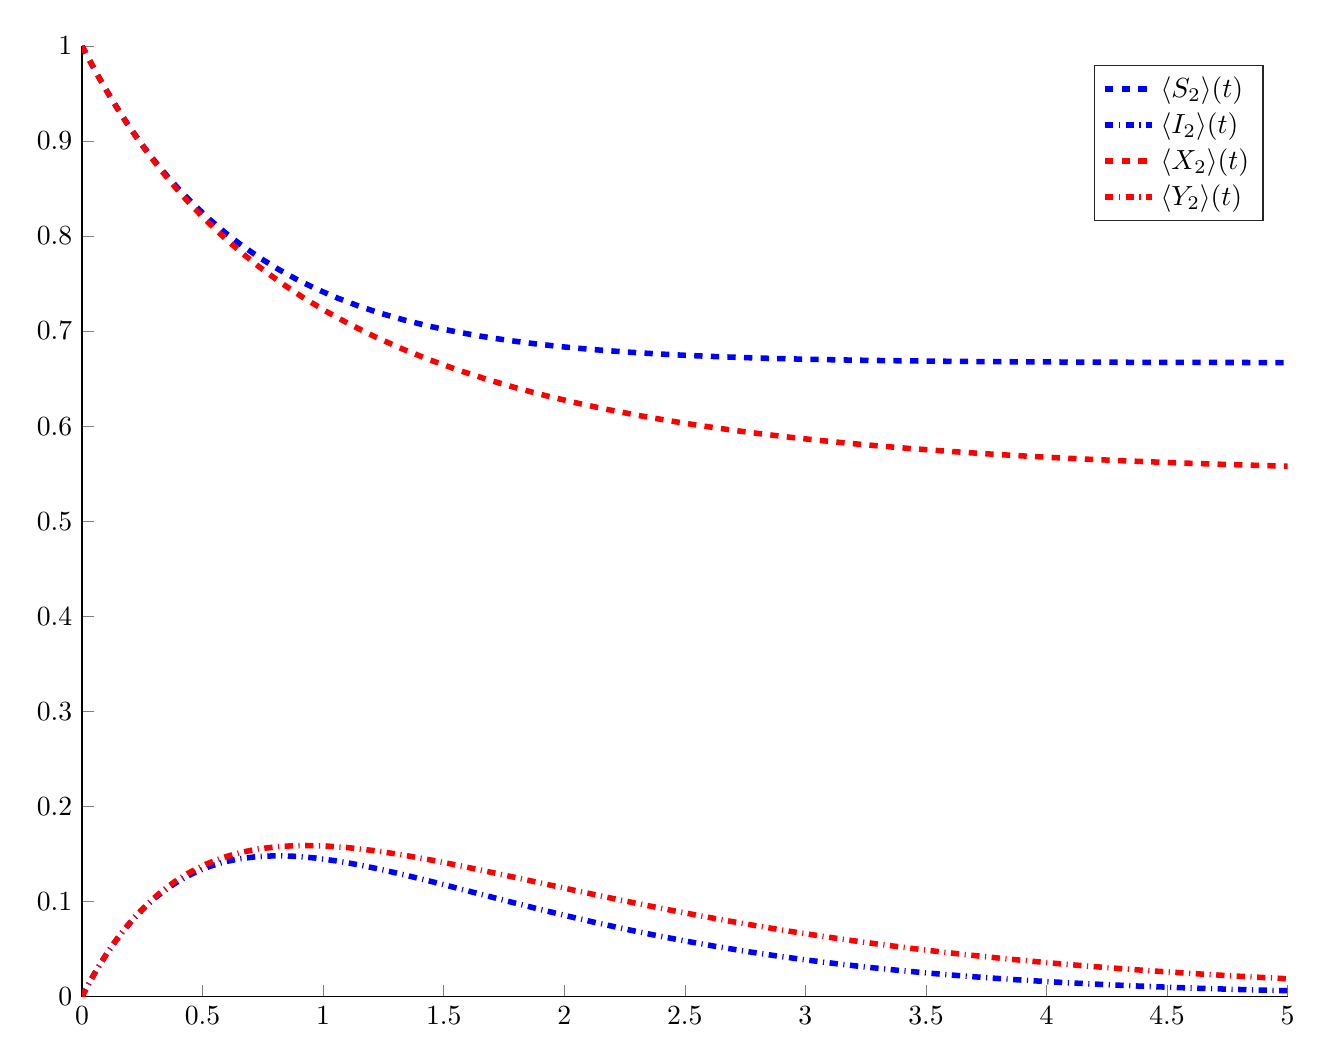
\begin{tikzpicture}

\begin{axis}[%
width=6.028in,
height=4.754in,
at={(1.011in,0.642in)},
scale only axis,
xmin=0,
xmax=5,
ymin=0,
ymax=1,
axis background/.style={fill=white},
axis x line*=bottom,
axis y line*=left,
legend style={legend cell align=left, align=left, draw=white!15!black}
]
\addplot [color=blue, dashed, line width=2.0pt]
  table[row sep=crcr]{%
0	1\\
0.000100475457260383	0.999949766056924\\
0.000200950914520766	0.999899539684195\\
0.00030142637178115	0.999849320880672\\
0.000401901829041533	0.999799109645214\\
0.000904279115343449	0.999548166948998\\
0.00140665640164536	0.999297413283416\\
0.00190903368794728	0.999046848506074\\
0.0024114109742492	0.998796472474686\\
0.00492329740575878	0.997547418534447\\
0.00743518383726836	0.996303061961732\\
0.00994707026877794	0.995063385091027\\
0.0124589567002875	0.993828370323048\\
0.0250183888578354	0.987722616365095\\
0.0375778210153833	0.981730813042634\\
0.0501372531729312	0.975850833944071\\
0.0626966853304791	0.970080591669277\\
0.0991412937643315	0.953939046011196\\
0.135585902198184	0.938656254473793\\
0.172030510632036	0.924186587013759\\
0.208475119065889	0.910486692796938\\
0.257093885813804	0.893338017841503\\
0.305712652561719	0.877395555845\\
0.354331419309635	0.862574680234777\\
0.40295018605755	0.848796177141757\\
0.46627950019307	0.832290618164177\\
0.52960881432859	0.817281114199863\\
0.592938128464109	0.803632751202841\\
0.656267442599629	0.791221205689014\\
0.733658471248229	0.777568429104202\\
0.811049499896829	0.765412570030883\\
0.888440528545428	0.754590931818442\\
0.965831557194028	0.744955370973288\\
1.05793596976172	0.734850994744874\\
1.15004038232942	0.726051284757239\\
1.24214479489711	0.718390163309227\\
1.3342492074648	0.711717689094676\\
1.44286725998794	0.704941359996623\\
1.55148531251107	0.699184906067961\\
1.66010336503421	0.694298310044978\\
1.76872141755734	0.690146590836533\\
1.88893196521442	0.68626979781265\\
2.00914251287149	0.683033580994597\\
2.12935306052856	0.680335328566429\\
2.24956360818563	0.678082495710856\\
2.37456360818563	0.676129062260638\\
2.49956360818563	0.67451015902841\\
2.62456360818563	0.673170462694345\\
2.74956360818563	0.672059963058475\\
2.87456360818563	0.6711370825968\\
2.99956360818563	0.670372247653384\\
3.12456360818563	0.669739321268742\\
3.24956360818563	0.669214676614722\\
3.37456360818563	0.668778670798171\\
3.49956360818563	0.66841733203559\\
3.62456360818563	0.668118312176992\\
3.74956360818563	0.667870448959301\\
3.87456360818563	0.66766446229043\\
3.99956360818563	0.667493751338391\\
4.12456360818563	0.667352482340913\\
4.24956360818563	0.667235381796357\\
4.37456360818563	0.667138065416295\\
4.49956360818563	0.667057414702439\\
4.62456360818563	0.666990673551059\\
4.74956360818563	0.666935350548061\\
4.81217270613922	0.666911265128768\\
4.87478180409282	0.666889339104704\\
4.93739090204641	0.666869379826172\\
5	0.66685120964227\\
};
\addlegendentry{$\langle\text{ S}_\text{2}\text{ }\rangle\text{(t)}$}

\addplot [color=blue, dashdotted, line width=2.0pt]
  table[row sep=crcr]{%
0	0\\
0.000100475457260383	5.02314194582358e-05\\
0.000200950914520766	0.000100450222178378\\
0.00030142637178115	0.000150656410568844\\
0.000401901829041533	0.000200849987037635\\
0.000904279115343449	0.000451628774807697\\
0.00140665640164536	0.00070209262549841\\
0.00190903368794728	0.000952241839644842\\
0.0024114109742492	0.00120207671752405\\
0.00492329740575878	0.00244654655480787\\
0.00743518383726836	0.00368320287872335\\
0.00994707026877794	0.00491208293452641\\
0.0124589567002875	0.0061332238082172\\
0.0250183888578354	0.0121241281424412\\
0.0375778210153833	0.0179270245694221\\
0.0501372531729312	0.0235463722993485\\
0.0626966853304791	0.02898653721096\\
0.0991412937643315	0.0437975780064231\\
0.135585902198184	0.0572353494401202\\
0.172030510632036	0.0693937083334257\\
0.208475119065889	0.0803611576950339\\
0.257093885813804	0.0932814625263713\\
0.305712652561719	0.104411444050903\\
0.354331419309635	0.113918297020974\\
0.40295018605755	0.121956876117229\\
0.46627950019307	0.130459773511127\\
0.52960881432859	0.13699148818833\\
0.592938128464109	0.141802573766275\\
0.656267442599629	0.145120569742411\\
0.733658471248229	0.147443262414491\\
0.811049499896829	0.148152783459638\\
0.888440528545428	0.147523537737773\\
0.965831557194028	0.145800614492561\\
1.05793596976172	0.14261761324062\\
1.15004038232942	0.138468469319266\\
1.24214479489711	0.133593199535327\\
1.3342492074648	0.128203232510097\\
1.44286725998794	0.121423706047034\\
1.55148531251107	0.114375584460389\\
1.66010336503421	0.10722364787831\\
1.76872141755734	0.100112083509218\\
1.88893196521442	0.0924224291243308\\
2.00914251287149	0.0850002476399585\\
2.12935306052856	0.0779076868343403\\
2.24956360818563	0.0711991011319526\\
2.37456360818563	0.0646673812660732\\
2.49956360818563	0.0585888424369925\\
2.62456360818563	0.0529600282470089\\
2.74956360818563	0.0477773110138708\\
2.87456360818563	0.0430297403451633\\
2.99956360818563	0.0386916182635999\\
3.12456360818563	0.0347385923849993\\
3.24956360818563	0.0311483438435658\\
3.37456360818563	0.0278975046540668\\
3.49956360818563	0.0249585909052709\\
3.62456360818563	0.0223063173817782\\
3.74956360818563	0.0199176420689963\\
3.87456360818563	0.0177704893156483\\
3.99956360818563	0.0158425684352806\\
4.12456360818563	0.0141135755002288\\
4.24956360818563	0.0125650442349459\\
4.37456360818563	0.0111798516748117\\
4.49956360818563	0.00994182226490993\\
4.62456360818563	0.0088362940755339\\
4.74956360818563	0.00784994516657192\\
4.81217270613922	0.00739687025071491\\
4.87478180409282	0.00696920095174279\\
4.93739090204641	0.00656558347103006\\
5	0.00618472765868362\\
};
\addlegendentry{$\langle\text{ I}_\text{2}\rangle\text{(t)}$}

\addplot [color=red, dashed, line width=2.0pt]
  table[row sep=crcr]{%
0	1\\
0.000100475457260383	0.99994976605686\\
0.000200950914520766	0.999899539683687\\
0.00030142637178115	0.999849320878961\\
0.000401901829041533	0.999799109641159\\
0.000904279115343449	0.99954816690284\\
0.00140665640164536	0.999297413109794\\
0.00190903368794728	0.999046848072382\\
0.0024114109742492	0.998796471601204\\
0.00492329740575878	0.997547411126232\\
0.00743518383726836	0.996303036533294\\
0.00994707026877794	0.995063324412706\\
0.0124589567002875	0.993828251500648\\
0.0250183888578354	0.987721670488083\\
0.0375778210153833	0.981727662789085\\
0.0501372531729312	0.975843478285104\\
0.0626966853304791	0.970066449874119\\
0.102108236390274	0.952605420168752\\
0.141519787450068	0.936099675314657\\
0.180931338509863	0.920480826836349\\
0.220342889569658	0.905686357257161\\
0.274870838360705	0.886471518613129\\
0.329398787151753	0.868591348141757\\
0.383926735942801	0.851925610206075\\
0.438454684733849	0.836366826263978\\
0.511698843017727	0.81704354767056\\
0.584943001301606	0.799345706541171\\
0.658187159585485	0.783098638750895\\
0.731431317869363	0.76814911627258\\
0.823962581336954	0.750913024428527\\
0.916493844804545	0.735311720644982\\
1.00902510827214	0.721151661167631\\
1.10155637173973	0.708264369444304\\
1.21569652246265	0.693908865254259\\
1.32983667318558	0.681051271536474\\
1.44397682390851	0.669502958947782\\
1.55811697463144	0.659099610029634\\
1.68311697463144	0.648856496917941\\
1.80811697463144	0.639673519417067\\
1.93311697463144	0.631422907332402\\
2.05811697463144	0.62399201116677\\
2.18311697463144	0.617284880263026\\
2.30811697463144	0.611222776938041\\
2.43311697463144	0.605735753729153\\
2.55811697463144	0.600761252574241\\
2.68311697463144	0.596244823027247\\
2.80811697463144	0.592140568132477\\
2.93311697463144	0.588407274158174\\
3.05811697463144	0.585007690098468\\
3.18311697463144	0.581908882003535\\
3.30811697463144	0.579082536837936\\
3.43311697463144	0.576503021741188\\
3.55811697463144	0.574146990158659\\
3.68311697463144	0.571993567402675\\
3.80811697463144	0.570024546403732\\
3.93311697463144	0.56822334343106\\
4.05811697463144	0.566574770310173\\
4.18311697463144	0.565065136603473\\
4.30811697463144	0.563682374949081\\
4.43311697463144	0.562415445174647\\
4.55811697463144	0.561254196069616\\
4.66858773097358	0.56030851506375\\
4.77905848731572	0.559432507092414\\
4.88952924365786	0.558620902201171\\
5	0.557868805996139\\
};
\addlegendentry{$\langle\text{ X}_\text{2}\rangle\text{(t)}$}

\addplot [color=red, dashdotted, line width=2.0pt]
  table[row sep=crcr]{%
0	0\\
0.000100475457260383	5.02314195216212e-05\\
0.000200950914520766	0.000100450222685378\\
0.00030142637178115	0.00015065641227969\\
0.000401901829041533	0.000200849991092313\\
0.000904279115343449	0.000451628820955347\\
0.00140665640164536	0.000702092799059145\\
0.00190903368794728	0.000952242273129502\\
0.0024114109742492	0.00120207759047991\\
0.00492329740575878	0.00244655395390654\\
0.00743518383726836	0.00368322825984696\\
0.00994707026877794	0.00491214346181296\\
0.0124589567002875	0.00613334226017403\\
0.0250183888578354	0.0121250680925129\\
0.0375778210153833	0.0179301450594698\\
0.0501372531729312	0.023553635330364\\
0.0626966853304791	0.0290004563591362\\
0.102108236390274	0.044998106770484\\
0.141519787450068	0.0594409659043847\\
0.180931338509863	0.0724560696360787\\
0.220342889569658	0.0841600869174819\\
0.274870838360705	0.0983885821787152\\
0.329398787151753	0.110563341086724\\
0.383926735942801	0.120909930751128\\
0.438454684733849	0.129630673618899\\
0.511698843017727	0.139099340842715\\
0.584943001301606	0.14633229027685\\
0.658187159585485	0.151654455741052\\
0.731431317869363	0.155350568031261\\
0.823962581336954	0.158073528446468\\
0.916493844804545	0.158994675694103\\
1.00902510827214	0.158455276740108\\
1.10155637173973	0.15674915749057\\
1.21569652246265	0.153397558084643\\
1.32983667318558	0.148992022221842\\
1.44397682390851	0.14381988595314\\
1.55811697463144	0.138124909820625\\
1.68311697463144	0.131515619398056\\
1.80811697463144	0.124686585141643\\
1.93311697463144	0.117780309428003\\
2.05811697463144	0.110915874064973\\
2.18311697463144	0.10418236746683\\
2.30811697463144	0.097633998120614\\
2.43311697463144	0.0913133288412923\\
2.55811697463144	0.0852540775432535\\
2.68311697463144	0.0794782645069583\\
2.80811697463144	0.0739939269600281\\
2.93311697463144	0.068804964989228\\
3.05811697463144	0.0639123325840836\\
3.18311697463144	0.0593127662216291\\
3.30811697463144	0.0549977514099881\\
3.43311697463144	0.0509577192898392\\
3.55811697463144	0.0471825185717931\\
3.68311697463144	0.0436608459305459\\
3.80811697463144	0.0403798026923218\\
3.93311697463144	0.0373266305829282\\
4.05811697463144	0.0344888684754468\\
4.18311697463144	0.0318541013086588\\
4.30811697463144	0.0294097888400823\\
4.43311697463144	0.027143921496779\\
4.55811697463144	0.025045044993035\\
4.66858773097358	0.02332031744584\\
4.77905848731572	0.0217100684354412\\
4.88952924365786	0.0202073223544393\\
5	0.0188054435162205\\
};
\addlegendentry{$\langle\text{ Y}_\text{2}\rangle\text{(t)}$}

\end{axis}
\end{tikzpicture}%}}
\\
\subfloat[][Nodo 3]
{\resizebox{0.45\textwidth}{!}
{% This file was created by matlab2tikz.
%
%The latest updates can be retrieved from
%  http://www.mathworks.com/matlabcentral/fileexchange/22022-matlab2tikz-matlab2tikz
%where you can also make suggestions and rate matlab2tikz.
%
\begin{tikzpicture}

\begin{axis}[%
width=6.028in,
height=4.754in,
at={(1.011in,0.642in)},
scale only axis,
xmin=0,
xmax=5,
ymin=0,
ymax=1,
axis background/.style={fill=white},
axis x line*=bottom,
axis y line*=left,
legend style={legend cell align=left, align=left, draw=white!15!black}
]
\addplot [color=blue, dashed, line width=2.0pt]
  table[row sep=crcr]{%
0	1\\
0.000100475457260383	0.999999998738212\\
0.000200950914520766	0.999999994953355\\
0.00030142637178115	0.999999988646191\\
0.000401901829041533	0.999999979817478\\
0.000904279115343449	0.999999897877294\\
0.00140665640164536	0.999999753012362\\
0.00190903368794728	0.999999545317527\\
0.0024114109742492	0.999999274887529\\
0.00492329740575878	0.999996985018619\\
0.00743518383726836	0.999993140920042\\
0.00994707026877794	0.999987754314207\\
0.0124589567002875	0.999980836857604\\
0.0250183888578354	0.99992369060678\\
0.0375778210153833	0.999829983819626\\
0.0501372531729312	0.999701100729764\\
0.0626966853304791	0.999538387544353\\
0.0991412937643315	0.998886739620121\\
0.135585902198184	0.997991230171454\\
0.172030510632036	0.996879570264252\\
0.208475119065889	0.995577412935433\\
0.257093885813804	0.993584304544217\\
0.305712652561719	0.991343692722487\\
0.354331419309635	0.988899958766603\\
0.40295018605755	0.986293161164884\\
0.46627950019307	0.982711525512293\\
0.52960881432859	0.978978851029841\\
0.592938128464109	0.975151047644084\\
0.656267442599629	0.971277107477869\\
0.733658471248229	0.966540180123668\\
0.811049499896829	0.96185148231486\\
0.888440528545428	0.957255674274212\\
0.965831557194028	0.952790640795762\\
1.05793596976172	0.947687158789251\\
1.15004038232942	0.942836240127123\\
1.24214479489711	0.938255225417784\\
1.3342492074648	0.93395785105292\\
1.44286725998794	0.929263154252068\\
1.55148531251107	0.924960889826022\\
1.66010336503421	0.921036164290667\\
1.76872141755734	0.917475682986413\\
1.88893196521442	0.913939116138171\\
2.00914251287149	0.910791072241598\\
2.12935306052856	0.90799748690281\\
2.24956360818563	0.905529099198296\\
2.37456360818563	0.903276215029636\\
2.49956360818563	0.901307177075887\\
2.62456360818563	0.899589947309379\\
2.74956360818563	0.898096741698768\\
2.87456360818563	0.896802006580401\\
2.99956360818563	0.895680825314712\\
3.12456360818563	0.894711537182946\\
3.24956360818563	0.89387511783864\\
3.37456360818563	0.893154591175261\\
3.49956360818563	0.892534697742382\\
3.62456360818563	0.89200212163112\\
3.74956360818563	0.891545088498192\\
3.87456360818563	0.891153261524557\\
3.99956360818563	0.890817783742232\\
4.12456360818563	0.890530907876842\\
4.24956360818563	0.890285754811511\\
4.37456360818563	0.890076346551204\\
4.49956360818563	0.889897720225924\\
4.62456360818563	0.889745527695439\\
4.74956360818563	0.889615897047471\\
4.81217270613922	0.889558385188113\\
4.87478180409282	0.889505342645769\\
4.93739090204641	0.889456431138355\\
5	0.889411335108728\\
};
\addlegendentry{$\langle\text{ S}_\text{3}\rangle\text{(t)}$}

\addplot [color=blue, dashdotted, line width=2.0pt]
  table[row sep=crcr]{%
0	0\\
0.000100475457260383	1.26174564507511e-09\\
0.000200950914520766	5.04630649619944e-09\\
0.00030142637178115	1.13526686325144e-08\\
0.000401901829041533	2.01798184068852e-08\\
0.000904279115343449	1.02091923284483e-07\\
0.00140665640164536	2.46871829401846e-07\\
0.00190903368794728	4.54393138543501e-07\\
0.0024114109742492	7.24529622981851e-07\\
0.00492329740575878	3.01003339887932e-06\\
0.00743518383726836	6.84208032837421e-06\\
0.00994707026877794	1.22050829335585e-05\\
0.0124589567002875	1.90835584530528e-05\\
0.0250183888578354	7.56726871955182e-05\\
0.0375778210153833	0.000167886153179433\\
0.0501372531729312	0.000293904054128181\\
0.0626966853304791	0.000451966247176856\\
0.0991412937643315	0.00107640515725554\\
0.135585902198184	0.00191791339955295\\
0.172030510632036	0.00294158455442854\\
0.208475119065889	0.00411561168567354\\
0.257093885813804	0.00586656673522458\\
0.305712652561719	0.00777592172844151\\
0.354331419309635	0.00979310095594282\\
0.40295018605755	0.011873569764334\\
0.46627950019307	0.0146158151384264\\
0.52960881432859	0.0173360492986682\\
0.592938128464109	0.0199821820368625\\
0.656267442599629	0.0225104529978181\\
0.733658471248229	0.02539115114769\\
0.811049499896829	0.0280109065459407\\
0.888440528545428	0.0303474467335782\\
0.965831557194028	0.0323840630785625\\
1.05793596976172	0.0344071316177395\\
1.15004038232942	0.0360110336951349\\
1.24214479489711	0.0372176865912015\\
1.3342492074648	0.0380473684460118\\
1.44286725998794	0.0385756032874527\\
1.55148531251107	0.0386778210502849\\
1.66010336503421	0.0384134650512885\\
1.76872141755734	0.0378316253865122\\
1.88893196521442	0.0368748785224682\\
2.00914251287149	0.0356606119097609\\
2.12935306052856	0.0342505546923396\\
2.24956360818563	0.0326942992479208\\
2.37456360818563	0.030967798437803\\
2.49956360818563	0.0291774702377419\\
2.62456360818563	0.0273606490132158\\
2.74956360818563	0.0255470489760419\\
2.87456360818563	0.0237608032007619\\
2.99956360818563	0.022021389972849\\
3.12456360818563	0.0203433021049032\\
3.24956360818563	0.0187376669423681\\
3.37456360818563	0.0172124019264551\\
3.49956360818563	0.0157718297137138\\
3.62456360818563	0.0144182646654105\\
3.74956360818563	0.0131528255337223\\
3.87456360818563	0.0119751670324062\\
3.99956360818563	0.0108829685469754\\
4.12456360818563	0.00987333421061613\\
4.24956360818563	0.00894316159677071\\
4.37456360818563	0.00808887743749468\\
4.49956360818563	0.00730607628957589\\
4.62456360818563	0.00659038454027418\\
4.74956360818563	0.00593760457221872\\
4.81217270613922	0.00563297981514419\\
4.87478180409282	0.00534251211914012\\
4.93739090204641	0.00506566988213707\\
5	0.00480193197476929\\
};
\addlegendentry{$\langle\text{ I}_\text{3}\rangle\text{(t)}$}

\addplot [color=red, dashed, line width=2.0pt]
  table[row sep=crcr]{%
0	1\\
0.000100475457260383	0.999999998738191\\
0.000200950914520766	0.999999994953186\\
0.00030142637178115	0.99999998864562\\
0.000401901829041533	0.999999979816126\\
0.000904279115343449	0.999999897861903\\
0.00140665640164536	0.999999752954457\\
0.00190903368794728	0.999999545172859\\
0.0024114109742492	0.999999274596105\\
0.00492329740575878	0.99999698254461\\
0.00743518383726836	0.999993132420151\\
0.00994707026877794	0.999987734012498\\
0.0124589567002875	0.99998079706479\\
0.0250183888578354	0.999923372193665\\
0.0375778210153833	0.999828918556151\\
0.0501372531729312	0.999698602265756\\
0.0626966853304791	0.999533561935855\\
0.102108236390274	0.998802473641527\\
0.141519787450068	0.997772802574252\\
0.180931338509863	0.996474686254043\\
0.220342889569658	0.994936097629084\\
0.274870838360705	0.992458625188096\\
0.329398787151753	0.989631478470949\\
0.383926735942801	0.986509636921053\\
0.438454684733849	0.983142521239225\\
0.511698843017727	0.978310172298379\\
0.584943001301606	0.973204600176662\\
0.658187159585485	0.967903108385807\\
0.731431317869363	0.96247238848309\\
0.823962581336954	0.955513417925539\\
0.916493844804545	0.948525556772722\\
1.00902510827214	0.941579837962897\\
1.10155637173973	0.93473457001495\\
1.21569652246265	0.926495384374746\\
1.32983667318558	0.918532690985799\\
1.44397682390851	0.910885669360118\\
1.55811697463144	0.903583379985585\\
1.68311697463144	0.896001599857546\\
1.80811697463144	0.888856841971558\\
1.93311697463144	0.88214616617151\\
2.05811697463144	0.875863390315864\\
2.18311697463144	0.869997039523815\\
2.30811697463144	0.864528763069464\\
2.43311697463144	0.859439757644224\\
2.55811697463144	0.854711385392399\\
2.68311697463144	0.850324228182814\\
2.80811697463144	0.846257282913509\\
2.93311697463144	0.842490434993676\\
3.05811697463144	0.839004605341035\\
3.18311697463144	0.83578132135176\\
3.30811697463144	0.832802338556694\\
3.43311697463144	0.830050513428598\\
3.55811697463144	0.827509791402435\\
3.68311697463144	0.825165017436687\\
3.80811697463144	0.823001775336086\\
3.93311697463144	0.821006622000955\\
4.05811697463144	0.819167029630726\\
4.18311697463144	0.817471306673834\\
4.30811697463144	0.815908541909835\\
4.43311697463144	0.814468596894661\\
4.55811697463144	0.813142043031549\\
4.66858773097358	0.812057056123539\\
4.77905848731572	0.811048192431131\\
4.88952924365786	0.810110210904377\\
5	0.809238201829634\\
};
\addlegendentry{$\langle\text{ X}_\text{3}\rangle\text{(t)}$}

\addplot [color=red, dashdotted, line width=2.0pt]
  table[row sep=crcr]{%
0	0\\
0.000100475457260383	1.26176677433918e-09\\
0.000200950914520766	5.04647550902712e-09\\
0.00030142637178115	1.13532389791388e-08\\
0.000401901829041533	2.01811701698418e-08\\
0.000904279115343449	1.02107311071931e-07\\
0.00140665640164536	2.46929713547395e-07\\
0.00190903368794728	4.54537736934869e-07\\
0.0024114109742492	7.24820871514549e-07\\
0.00492329740575878	3.01250438824467e-06\\
0.00743518383726836	6.85056445746801e-06\\
0.00994707026877794	1.22253341732314e-05\\
0.0124589567002875	1.9123227323487e-05\\
0.0250183888578354	7.59891947797722e-05\\
0.0375778210153833	0.000168941537870823\\
0.0501372531729312	0.000296371259182916\\
0.0626966853304791	0.000456716223900398\\
0.102108236390274	0.00115686811222818\\
0.141519787450068	0.00212267378585917\\
0.180931338509863	0.00331439394648711\\
0.220342889569658	0.00469576342697509\\
0.274870838360705	0.00685907963655639\\
0.329398787151753	0.00924777752682902\\
0.383926735942801	0.0117967025688062\\
0.438454684733849	0.0144488538513655\\
0.511698843017727	0.0180890012685514\\
0.584943001301606	0.021735359993018\\
0.658187159585485	0.0253139024212412\\
0.731431317869363	0.0287639749883468\\
0.823962581336954	0.0328675778482622\\
0.916493844804545	0.0366360238924908\\
1.00902510827214	0.0400328394824937\\
1.10155637173973	0.0430332462888488\\
1.21569652246265	0.0461737039673331\\
1.32983667318558	0.0487141702730558\\
1.44397682390851	0.0506846515289764\\
1.55811697463144	0.0521168921282875\\
1.68311697463144	0.0531151075724693\\
1.80811697463144	0.0535852918569844\\
1.93311697463144	0.0535933407761544\\
2.05811697463144	0.0531985381246195\\
2.18311697463144	0.0524581406890982\\
2.30811697463144	0.0514306135674018\\
2.43311697463144	0.0501674624766716\\
2.55811697463144	0.048714017741547\\
2.68311697463144	0.0471109819326109\\
2.80811697463144	0.045395383432091\\
2.93311697463144	0.0435992007703931\\
3.05811697463144	0.0417501338548236\\
3.18311697463144	0.0398720373222307\\
3.30811697463144	0.037985060603455\\
3.43311697463144	0.0361061900628175\\
3.55811697463144	0.0342498163757724\\
3.68311697463144	0.0324277842944738\\
3.80811697463144	0.0306492844874422\\
3.93311697463144	0.0289217080248439\\
4.05811697463144	0.0272510170259292\\
4.18311697463144	0.0256416835909181\\
4.30811697463144	0.0240965404869059\\
4.43311697463144	0.0226174901788106\\
4.55811697463144	0.0212057298762751\\
4.66858773097358	0.0200144148955584\\
4.77905848731572	0.0188756664203282\\
4.88952924365786	0.0177889231960149\\
5	0.0167534213015026\\
};
\addlegendentry{$\langle\text{ Y}_\text{3}\rangle\text{(t)}$}

\end{axis}
\end{tikzpicture}%}
}
\quad
\subfloat[][Prevalenza]
{\resizebox{0.45\textwidth}{!}
{% This file was created by matlab2tikz.
%
%The latest updates can be retrieved from
%  http://www.mathworks.com/matlabcentral/fileexchange/22022-matlab2tikz-matlab2tikz
%where you can also make suggestions and rate matlab2tikz.
%
\begin{tikzpicture}

\begin{axis}[%
width=6.028in,
height=4.754in,
at={(1.011in,0.642in)},
scale only axis,
xmin=0,
xmax=5,
ymin=0,
ymax=1,
axis background/.style={fill=white},
axis x line*=bottom,
axis y line*=left,
legend style={legend cell align=left, align=left, draw=white!15!black}
]
\addplot [color=blue, dashed, line width=2.0pt]
  table[row sep=crcr]{%
0	1\\
0.000100475457260383	0.999999998738212\\
0.000200950914520766	0.999999994953355\\
0.00030142637178115	0.999999988646191\\
0.000401901829041533	0.999999979817478\\
0.000904279115343449	0.999999897877294\\
0.00140665640164536	0.999999753012362\\
0.00190903368794728	0.999999545317527\\
0.0024114109742492	0.999999274887529\\
0.00492329740575878	0.999996985018619\\
0.00743518383726836	0.999993140920042\\
0.00994707026877794	0.999987754314207\\
0.0124589567002875	0.999980836857604\\
0.0250183888578354	0.99992369060678\\
0.0375778210153833	0.999829983819626\\
0.0501372531729312	0.999701100729764\\
0.0626966853304791	0.999538387544353\\
0.0991412937643315	0.998886739620121\\
0.135585902198184	0.997991230171454\\
0.172030510632036	0.996879570264252\\
0.208475119065889	0.995577412935433\\
0.257093885813804	0.993584304544217\\
0.305712652561719	0.991343692722487\\
0.354331419309635	0.988899958766603\\
0.40295018605755	0.986293161164884\\
0.46627950019307	0.982711525512293\\
0.52960881432859	0.978978851029841\\
0.592938128464109	0.975151047644084\\
0.656267442599629	0.971277107477869\\
0.733658471248229	0.966540180123668\\
0.811049499896829	0.96185148231486\\
0.888440528545428	0.957255674274212\\
0.965831557194028	0.952790640795762\\
1.05793596976172	0.947687158789251\\
1.15004038232942	0.942836240127123\\
1.24214479489711	0.938255225417784\\
1.3342492074648	0.93395785105292\\
1.44286725998794	0.929263154252068\\
1.55148531251107	0.924960889826022\\
1.66010336503421	0.921036164290667\\
1.76872141755734	0.917475682986413\\
1.88893196521442	0.913939116138171\\
2.00914251287149	0.910791072241598\\
2.12935306052856	0.90799748690281\\
2.24956360818563	0.905529099198296\\
2.37456360818563	0.903276215029636\\
2.49956360818563	0.901307177075887\\
2.62456360818563	0.899589947309379\\
2.74956360818563	0.898096741698768\\
2.87456360818563	0.896802006580401\\
2.99956360818563	0.895680825314712\\
3.12456360818563	0.894711537182946\\
3.24956360818563	0.89387511783864\\
3.37456360818563	0.893154591175261\\
3.49956360818563	0.892534697742382\\
3.62456360818563	0.89200212163112\\
3.74956360818563	0.891545088498192\\
3.87456360818563	0.891153261524557\\
3.99956360818563	0.890817783742232\\
4.12456360818563	0.890530907876842\\
4.24956360818563	0.890285754811511\\
4.37456360818563	0.890076346551204\\
4.49956360818563	0.889897720225924\\
4.62456360818563	0.889745527695439\\
4.74956360818563	0.889615897047471\\
4.81217270613922	0.889558385188113\\
4.87478180409282	0.889505342645769\\
4.93739090204641	0.889456431138355\\
5	0.889411335108728\\
};
\addlegendentry{$\langle\text{ S}_\text{3}\rangle\text{(t)}$}

\addplot [color=blue, dashdotted, line width=2.0pt]
  table[row sep=crcr]{%
0	0\\
0.000100475457260383	1.26174564507511e-09\\
0.000200950914520766	5.04630649619944e-09\\
0.00030142637178115	1.13526686325144e-08\\
0.000401901829041533	2.01798184068852e-08\\
0.000904279115343449	1.02091923284483e-07\\
0.00140665640164536	2.46871829401846e-07\\
0.00190903368794728	4.54393138543501e-07\\
0.0024114109742492	7.24529622981851e-07\\
0.00492329740575878	3.01003339887932e-06\\
0.00743518383726836	6.84208032837421e-06\\
0.00994707026877794	1.22050829335585e-05\\
0.0124589567002875	1.90835584530528e-05\\
0.0250183888578354	7.56726871955182e-05\\
0.0375778210153833	0.000167886153179433\\
0.0501372531729312	0.000293904054128181\\
0.0626966853304791	0.000451966247176856\\
0.0991412937643315	0.00107640515725554\\
0.135585902198184	0.00191791339955295\\
0.172030510632036	0.00294158455442854\\
0.208475119065889	0.00411561168567354\\
0.257093885813804	0.00586656673522458\\
0.305712652561719	0.00777592172844151\\
0.354331419309635	0.00979310095594282\\
0.40295018605755	0.011873569764334\\
0.46627950019307	0.0146158151384264\\
0.52960881432859	0.0173360492986682\\
0.592938128464109	0.0199821820368625\\
0.656267442599629	0.0225104529978181\\
0.733658471248229	0.02539115114769\\
0.811049499896829	0.0280109065459407\\
0.888440528545428	0.0303474467335782\\
0.965831557194028	0.0323840630785625\\
1.05793596976172	0.0344071316177395\\
1.15004038232942	0.0360110336951349\\
1.24214479489711	0.0372176865912015\\
1.3342492074648	0.0380473684460118\\
1.44286725998794	0.0385756032874527\\
1.55148531251107	0.0386778210502849\\
1.66010336503421	0.0384134650512885\\
1.76872141755734	0.0378316253865122\\
1.88893196521442	0.0368748785224682\\
2.00914251287149	0.0356606119097609\\
2.12935306052856	0.0342505546923396\\
2.24956360818563	0.0326942992479208\\
2.37456360818563	0.030967798437803\\
2.49956360818563	0.0291774702377419\\
2.62456360818563	0.0273606490132158\\
2.74956360818563	0.0255470489760419\\
2.87456360818563	0.0237608032007619\\
2.99956360818563	0.022021389972849\\
3.12456360818563	0.0203433021049032\\
3.24956360818563	0.0187376669423681\\
3.37456360818563	0.0172124019264551\\
3.49956360818563	0.0157718297137138\\
3.62456360818563	0.0144182646654105\\
3.74956360818563	0.0131528255337223\\
3.87456360818563	0.0119751670324062\\
3.99956360818563	0.0108829685469754\\
4.12456360818563	0.00987333421061613\\
4.24956360818563	0.00894316159677071\\
4.37456360818563	0.00808887743749468\\
4.49956360818563	0.00730607628957589\\
4.62456360818563	0.00659038454027418\\
4.74956360818563	0.00593760457221872\\
4.81217270613922	0.00563297981514419\\
4.87478180409282	0.00534251211914012\\
4.93739090204641	0.00506566988213707\\
5	0.00480193197476929\\
};
\addlegendentry{$\langle\text{ I}_\text{3}\rangle\text{(t)}$}

\addplot [color=red, dashed, line width=2.0pt]
  table[row sep=crcr]{%
0	1\\
0.000100475457260383	0.999999998738191\\
0.000200950914520766	0.999999994953186\\
0.00030142637178115	0.99999998864562\\
0.000401901829041533	0.999999979816126\\
0.000904279115343449	0.999999897861903\\
0.00140665640164536	0.999999752954457\\
0.00190903368794728	0.999999545172859\\
0.0024114109742492	0.999999274596105\\
0.00492329740575878	0.99999698254461\\
0.00743518383726836	0.999993132420151\\
0.00994707026877794	0.999987734012498\\
0.0124589567002875	0.99998079706479\\
0.0250183888578354	0.999923372193665\\
0.0375778210153833	0.999828918556151\\
0.0501372531729312	0.999698602265756\\
0.0626966853304791	0.999533561935855\\
0.102108236390274	0.998802473641527\\
0.141519787450068	0.997772802574252\\
0.180931338509863	0.996474686254043\\
0.220342889569658	0.994936097629084\\
0.274870838360705	0.992458625188096\\
0.329398787151753	0.989631478470949\\
0.383926735942801	0.986509636921053\\
0.438454684733849	0.983142521239225\\
0.511698843017727	0.978310172298379\\
0.584943001301606	0.973204600176662\\
0.658187159585485	0.967903108385807\\
0.731431317869363	0.96247238848309\\
0.823962581336954	0.955513417925539\\
0.916493844804545	0.948525556772722\\
1.00902510827214	0.941579837962897\\
1.10155637173973	0.93473457001495\\
1.21569652246265	0.926495384374746\\
1.32983667318558	0.918532690985799\\
1.44397682390851	0.910885669360118\\
1.55811697463144	0.903583379985585\\
1.68311697463144	0.896001599857546\\
1.80811697463144	0.888856841971558\\
1.93311697463144	0.88214616617151\\
2.05811697463144	0.875863390315864\\
2.18311697463144	0.869997039523815\\
2.30811697463144	0.864528763069464\\
2.43311697463144	0.859439757644224\\
2.55811697463144	0.854711385392399\\
2.68311697463144	0.850324228182814\\
2.80811697463144	0.846257282913509\\
2.93311697463144	0.842490434993676\\
3.05811697463144	0.839004605341035\\
3.18311697463144	0.83578132135176\\
3.30811697463144	0.832802338556694\\
3.43311697463144	0.830050513428598\\
3.55811697463144	0.827509791402435\\
3.68311697463144	0.825165017436687\\
3.80811697463144	0.823001775336086\\
3.93311697463144	0.821006622000955\\
4.05811697463144	0.819167029630726\\
4.18311697463144	0.817471306673834\\
4.30811697463144	0.815908541909835\\
4.43311697463144	0.814468596894661\\
4.55811697463144	0.813142043031549\\
4.66858773097358	0.812057056123539\\
4.77905848731572	0.811048192431131\\
4.88952924365786	0.810110210904377\\
5	0.809238201829634\\
};
\addlegendentry{$\langle\text{ X}_\text{3}\rangle\text{(t)}$}

\addplot [color=red, dashdotted, line width=2.0pt]
  table[row sep=crcr]{%
0	0\\
0.000100475457260383	1.26176677433918e-09\\
0.000200950914520766	5.04647550902712e-09\\
0.00030142637178115	1.13532389791388e-08\\
0.000401901829041533	2.01811701698418e-08\\
0.000904279115343449	1.02107311071931e-07\\
0.00140665640164536	2.46929713547395e-07\\
0.00190903368794728	4.54537736934869e-07\\
0.0024114109742492	7.24820871514549e-07\\
0.00492329740575878	3.01250438824467e-06\\
0.00743518383726836	6.85056445746801e-06\\
0.00994707026877794	1.22253341732314e-05\\
0.0124589567002875	1.9123227323487e-05\\
0.0250183888578354	7.59891947797722e-05\\
0.0375778210153833	0.000168941537870823\\
0.0501372531729312	0.000296371259182916\\
0.0626966853304791	0.000456716223900398\\
0.102108236390274	0.00115686811222818\\
0.141519787450068	0.00212267378585917\\
0.180931338509863	0.00331439394648711\\
0.220342889569658	0.00469576342697509\\
0.274870838360705	0.00685907963655639\\
0.329398787151753	0.00924777752682902\\
0.383926735942801	0.0117967025688062\\
0.438454684733849	0.0144488538513655\\
0.511698843017727	0.0180890012685514\\
0.584943001301606	0.021735359993018\\
0.658187159585485	0.0253139024212412\\
0.731431317869363	0.0287639749883468\\
0.823962581336954	0.0328675778482622\\
0.916493844804545	0.0366360238924908\\
1.00902510827214	0.0400328394824937\\
1.10155637173973	0.0430332462888488\\
1.21569652246265	0.0461737039673331\\
1.32983667318558	0.0487141702730558\\
1.44397682390851	0.0506846515289764\\
1.55811697463144	0.0521168921282875\\
1.68311697463144	0.0531151075724693\\
1.80811697463144	0.0535852918569844\\
1.93311697463144	0.0535933407761544\\
2.05811697463144	0.0531985381246195\\
2.18311697463144	0.0524581406890982\\
2.30811697463144	0.0514306135674018\\
2.43311697463144	0.0501674624766716\\
2.55811697463144	0.048714017741547\\
2.68311697463144	0.0471109819326109\\
2.80811697463144	0.045395383432091\\
2.93311697463144	0.0435992007703931\\
3.05811697463144	0.0417501338548236\\
3.18311697463144	0.0398720373222307\\
3.30811697463144	0.037985060603455\\
3.43311697463144	0.0361061900628175\\
3.55811697463144	0.0342498163757724\\
3.68311697463144	0.0324277842944738\\
3.80811697463144	0.0306492844874422\\
3.93311697463144	0.0289217080248439\\
4.05811697463144	0.0272510170259292\\
4.18311697463144	0.0256416835909181\\
4.30811697463144	0.0240965404869059\\
4.43311697463144	0.0226174901788106\\
4.55811697463144	0.0212057298762751\\
4.66858773097358	0.0200144148955584\\
4.77905848731572	0.0188756664203282\\
4.88952924365786	0.0177889231960149\\
5	0.0167534213015026\\
};
\addlegendentry{$\langle\text{ Y}_\text{3}\rangle\text{(t)}$}

\end{axis}
\end{tikzpicture}%}
}
\caption[Confronto tra modello esatto e chiuso alle coppie per~\ref{fig::3nodi}]{Nei grafici \`e possibile confrontare le soluzioni del modello esatto~\eqref{3nodi} (in blu) con il modello in cui abbiamo assunto l'indipendenza delle coppie~\eqref{Coppie3nodi} (in rosso)}
\label{fig::coppie3nodi}
\end{figure}
